\documentclass[11pt, oneside]{article} 
\usepackage{geometry}
\geometry{letterpaper} 
\usepackage{graphicx}
	
\usepackage{amssymb}
\usepackage{amsmath}
\usepackage{parskip}
\usepackage{color}
\usepackage{hyperref}

\graphicspath{{/Users/telliott_admin/Tex/png/}}
% \begin{center} 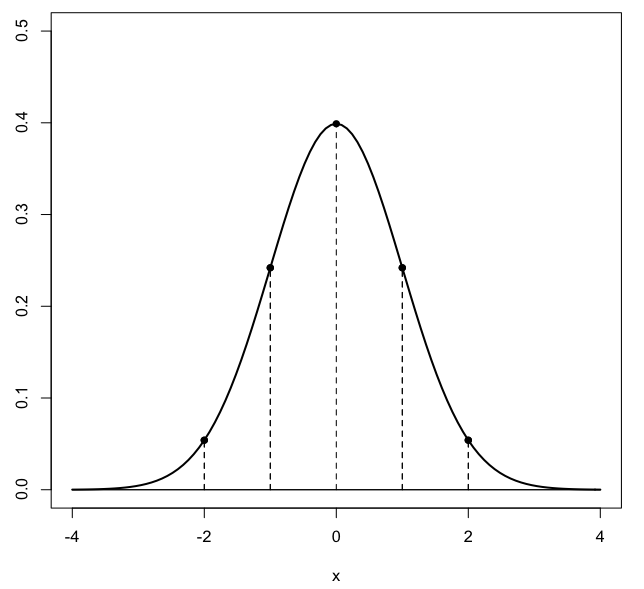
\includegraphics [scale=0.4] {gauss3.png} \end{center}

%break
\title{Projection}
\date{}

\begin{document}
\maketitle
\Large

We have two vectors $\mathbf{a}$ and $\mathbf{b}$ and we wish to find the component of $\mathbf{b}$ that is parallel to $\mathbf{a}$ (the projection of $\mathbf{b}$ on $\mathbf{a}$), as well as $\mathbf{e}$, the part that is perpendicular.  In this short writeup we will derive and use the equation, but let me just put it up here first:
\[ \mathbf{p} = \hat{x} \ \mathbf{a} = \frac{\mathbf{a} \cdot \mathbf{b} }{ \mathbf{a}\cdot \mathbf{a}} \  \mathbf{a} \]
The projection of $\mathbf{b}$ on $\mathbf{a}$ is just "$\mathbf{a}$ dot $\mathbf{b}$ over $\mathbf{a}$ dot $\mathbf{a}$, times $\mathbf{a}$."  

\begin{center}
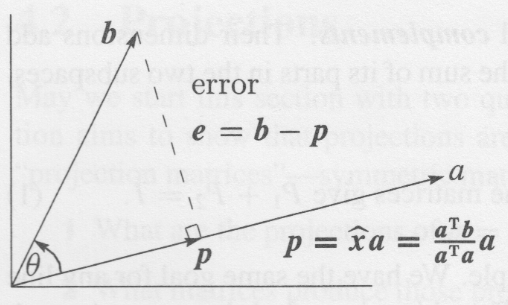
\includegraphics [scale=0.4] {projection.png}
\end{center}

We say that $\mathbf{p}$ is some multiple $\hat{x}$ of $\mathbf{a}$ 
\[ \mathbf{p} = \hat{x}\ \mathbf{a} \]
and that $\mathbf{b}$ is just the sum of $\mathbf{p} $ and $\mathbf{e} $
\[ \mathbf{p} + \mathbf{e} = \mathbf{b}, \ \ \ \  \mathbf{e} = \mathbf{b}- \mathbf{p} = \mathbf{b} - \hat{x} \ \mathbf{a}  \]
and then use perpendicularity
\[ \mathbf{a} \cdot \mathbf{e}  = 0 = \mathbf{a} \cdot(\mathbf{b}-\hat{x} \ \mathbf{a}) \]
\[ \hat{x} = \frac{\mathbf{a} \cdot \mathbf{b}}{ \mathbf{a}\cdot \mathbf{a}} \]
We can divide by $\mathbf{a} \cdot \mathbf{a}$ since it is just a number.  Finally
\[ \mathbf{p} = \hat{x}\ \mathbf{a} = \frac{\mathbf{a} \cdot \mathbf{b}}{ \mathbf{a}\cdot \mathbf{a}}  \mathbf{a}\]
Notice that the factor $\mathbf{a}\cdot \mathbf{a} = 1$ if $\mathbf{a}$ is a unit vector.  It's just a scaling factor.

Example 1.  Vector $b = \ <u,v>$, what is its projection on $i = \ <1,0>$?
\[ \hat{x} = \frac{a \cdot b}{ a\cdot a} = \frac{1 \times u + 0 \times v}{1 \times 1 + 0 \times 0} = u \]
So $p = ui = \ <u,0>$, as expected.
\[ e = a - p = \ <0,v> \]
\vspace{2 mm}

\noindent Example 2.  Vector $b = \ <3,1>$, what is its projection on $a = \ <1,1>$?
\[ \hat{x} = \frac{a \cdot b}{ a\cdot a} = \frac{1 \times 3 + 1 \times 1}{1 \times 1 + 1 \times 1} = \frac{4}{2} = 2 \]
\[ p = 2 \ <1,1> \ = \ <2,2> \]
The projection is $<2,2>$.
\[ e = b - p = \ <3,1> - <2,2> \ = \ <1,-1> \]
\[ p \cdot e = \ <2,2> \cdot <1,-1> \ =0 \]
Notice that the lengths work for a right triangle:
\[ \left| b \right|^2 = \left| p \right|^2 + \left| e \right|^2 \]
\[ 10 = 8 + 2 \]
This works for vectors in $\mathbb{R}^3$ as well.
\vspace{2 mm}

\noindent Example 3.  Vector $b = \ <3,4,4>$ and $a = \ <2,2,1>$.
\[ \hat{x} = \frac{a \cdot b}{ a\cdot a} = \frac{2 \times 3 + 2 \times 4 + 1 \times 4}{2 \times 2 + 2 \times 2 + 1 \times 1} = \frac{18}{9} = 2\]
\[ p = 2 \ <2,2,1> \ = \ <4,4,2> \]
\[ e = b-p =  \ <3,4,4> - <4,4,2> \ = \ <-1,0,2> \]
\[ e \cdot p = -4 + 4 = 0 \]

Now suppose that we add a second vector $a_2 = \ <1,0,0>$ (renaming the first one $a_1$).  And we ask to project $b$ onto the plane formed by $a_1$ and $a_2$.  Put the two vectors into a matrix A
\[A =
\begin{bmatrix} 
  a_1  &  a_2
\end{bmatrix}
=
\begin{bmatrix} 
  2  &  1   \\ 
  2  &  0  \\
  1  &  0
\end{bmatrix}
, \ \ \ \ 
b = 
\begin{bmatrix} 
  3   \\ 
  4   \\
  4
\end{bmatrix}
\]
The projection is some combination of the two vectors $a_1$ and $a_2$.
\[ p = \hat{x_1} a_1 + \hat{x_2} a_2 = A \hat{x} \]
We know that $e=b-p=b-A\hat{x}$ is $\perp$ to the plane.

\[ a_1^T(b-A \hat{x}) = 0 =  a_2^T(b-A \hat{x}) \]
Put them into a matrix
\[  
\begin{bmatrix} 
  a_1^T    \\ 
  a_2^T    \\
\end{bmatrix}
(b-A\hat{x}) =
\begin{bmatrix} 
  0    \\ 
  0    \\
\end{bmatrix}
\]
\[A^T(b-A\ \hat{x}) = 0 \]
\[A^T A\ \hat{x} = A^Tb \]
\[ \hat{x} = (A^T A)^{-1}A^Tb \]
The fundamental equation is then
\[ p = A \hat{x} = A(A^T A)^{-1}A^Tb \]
Compare with the one-dimensional case
\[ a\frac{a^Tb}{a^Ta} \]
Let's work the example
\[ A^T = 
\begin{bmatrix} 
  2  &  2  &  1   \\ 
  1  &  0  &  0   \\
\end{bmatrix}
\]
\[A^T A = 
\begin{bmatrix} 
  2  &  2  &  1   \\ 
  1  &  0  &  0   \\
\end{bmatrix}
\times
\begin{bmatrix} 
  2  &  1   \\ 
  2  &  0   \\
  1  &  0   \\
\end{bmatrix}
=
\begin{bmatrix} 
  9  &  2   \\ 
  2  &  1   \\
\end{bmatrix}
\]
\[ (A^T A)^{-1} = \frac{1}{5}
\begin{bmatrix} 
1  &  -2   \\ 
  -2  & 9   \\
\end{bmatrix}
\]
\[(A^T A)^{-1}A^T = \frac{1}{5} 
\begin{bmatrix} 
  0  &  2  &  1   \\ 
  5  &  -4  &  -2   \\
\end{bmatrix}
\]
And finally
\[P = A (A^T A)^{-1}A^T = \frac{1}{5} 
\begin{bmatrix} 
  5  &  0  &  0   \\ 
  0  &  4  &  2   \\
  0  &  2  &  1   \\
\end{bmatrix}
\]

\[ p = Pb = \frac{1}{5}
\begin{bmatrix} 
  5  &  0  &  0   \\ 
  0  &  4  &  2   \\
  0  &  2  &  1   \\
\end{bmatrix}
\begin{bmatrix} 
  3   \\ 
  4   \\
  4  
\end{bmatrix}
= \frac{1}{5} 
\begin{bmatrix} 
  15   \\ 
  24   \\
  12 
\end{bmatrix}
\]
\[
e = b - p =
\begin{bmatrix} 
  3   \\ 
  4   \\
  4 
\end{bmatrix}
-
\frac{1}{5} 
\begin{bmatrix} 
  15   \\ 
  24   \\
  12
\end{bmatrix}
=
\frac{1}{5} 
\begin{bmatrix} 
  0   \\ 
  -4   \\
  8 
\end{bmatrix}
\]
We should confirm both $a_1 \perp e$ and $a_2 \perp e$.
\[ <2,2,1> <0,-\frac{4}{5},\frac{8}{5}> \ = 0 \]
\[ <1,0,0> <0,-\frac{4}{5},\frac{8}{5}> \ = 0 \]

This problem can be made easier by using an orthonormal basis for the plane.  One such basis is obtained by finding the projection of $a_1$ on $a_2$ and subtracting that from $a_1$.  Since $a_2$ is a unit vector, the projection $p$ is just $<2,0,0>$ and the new basis vector $a_3$ (before normalization) is $<0,2,1>$.  The unit vector is $u = \ <0,2/\sqrt{5},1/\sqrt{5}>$.

Then
\[ A =
\begin{bmatrix} 
  0  &  1   \\ 
  2/\sqrt{5}  &  0   \\
  1/\sqrt{5}  &  0   \\
\end{bmatrix}
\]
and 
\[ A A^T = P = 
\begin{bmatrix} 
  0  &  1   \\ 
  2/\sqrt{5}  &  0   \\
  1/\sqrt{5}  &  0   \\
\end{bmatrix}
\begin{bmatrix} 
  0  &  2/\sqrt{5} & 1/\sqrt{5}   \\ 
  1  &  0 & 1  
\end{bmatrix}
\]
\[P  = 
\begin{bmatrix} 
  1  &  0 & 0   \\ 
  0  &  4/5 & 2/5   \\ 
  0  &  2/5 & 1/5
\end{bmatrix}
\]
We easily confirm that 
\[ P a_3 =
0 
\begin{bmatrix} 
  1   \\ 
  0    \\ 
  0
  \end{bmatrix}
+
2
\begin{bmatrix} 
  0   \\ 
  4/5    \\ 
  2/5
  \end{bmatrix}
+
1
\begin{bmatrix} 
  0   \\ 
  2/5    \\ 
  1/5
  \end{bmatrix}
= a_3 \]

And for that matter $P a_1=a_1$;  $P a_2=a_2$; and $P u=u$.

\subsection*{another way}
It is worth pointing out that there is another way to do this problem which avoids the matrix multiplications required above.  We first use the two vectors in the plane to find the normal vector, then find the projection of vector $b$ on it.  That is $e$.  Then we find $p$ by subtraction.

Remember the "determinant" trick for doing the cross-product
\[ 
\begin{bmatrix} 
  i  &  j  &  k   \\ 
  2  &  2  &  1   \\
  1  &  0  &  0   \\
\end{bmatrix}
\]
\[ n = \ <0,1,-2> \]
Check that $n \perp$ to both $a_1$ and $a_2$.  Now recall $b= \ <3,4,4>$ and do
\[ e = \frac{b \cdot n}{n \cdot n} n = -\frac{4}{5} \ <0,1,-2> \  = \frac{1}{5} \ <0,-4,8>\]
which matches what we got before!
\subsection*{last point}
Finally, note that the vectors we started with, $a_1 = \ <2,2,1>$ and $a_2 = \ <1,0,0>$ are eigenvectors of the projection matrix $P$ with eigenvalue $\lambda = 1$, since 
\[ P a_1 = a_1 \]
\[ P a_2 = a_2 \]
In fact, \emph{any} vector that is a linear combination of $a_1$ and $a_2$ (that lies in the plane), has this property.  Furthermore,
\[ P v = P P v \]
for all $v$.  Once a vector is projected into the plane, another projection doesn't change it.

\end{document}  